\chapter{Statistical treatment of searching for new particles or processes}
\label{sec:statisticalfit}

In the experiments of particle physics, one often searches for particles or processes that have been predicted but not yet observed, such as the two analysis presented in this dissertation: searching for the vector boson scattering process and searching for the heavy resonance(s).
Usually two hypotheses are defined:
\begin{itemize}
    \item $H_{0}$: null hypothesis, in most cases are designated as background-only hypothesis.
    \item $H_{1}$: signal plus background hypothesis, where signal is a new model one would like to search for.
\end{itemize}
For the purpose of discovering a new signal process, the $H_{0}$ hypothesis is tested against the alternative $H_{1}$.
When setting limits, the $H_{1}$ hypotheses with different signal strengths are tested against the $H_{0}$.

The level of agreement between observed data and a given hypothesis can be quantified by computing the $p$-value, the probability under this hypothesis assumption, or its equivalent Gaussian significance.
This section describes the statistical treatment for searches related to this dissertation.

\section{The likelihood function}

The likelihood function is defined as the product of a set of the probability density functions (pdfs) of variables $x$, that used to evaluate the probability of the observed dataset:
\begin{equation}\label{eq:likelihoodf}
    \mathcal{L} (x_{1}, ..., x_{N}; \theta_{1}, ..., \theta_{M}) = \prod_{i}^{N} f(x_{i}; \theta_{1}, ..., \theta_{M})
\end{equation}
where $\theta_{1}$, ..., $\theta_{M}$ are the nuisance parameters that can be written as $\pmb{\theta}$,
and $x_{1}$, ..., $x_{N}$ denote the observables of dataset. 
Usually one measures the variable $x$ by constructing a histogram $\pmb{n} = (n_{1}, ..., n_{N})$.
The expectation value of the ith bin $n_{i}$ is written as~\cite{Cowan:2010js}:
\begin{equation}\label{eq:discri}
    E[n_{i}] = \mu s_{i} + b_{i}
\end{equation}
where $\mu$ is the signal strength, $s_{i}$ and $b_{i}$ are the number of signal and background events in that bin.
In addition to the histogram $\pmb{n}$, in some cases, one would like to use subsidiary measurements to further constrain the nuisance parameters.
For instance, due to the lack of background simulation or the mismodelling issue of one MC sample, one can choose a control region and construct another histogram $\pmb{m} = (m_{1}, ..., m_{M})$ to constrain the contribution of one certain background in data.
For this measurement, the expectation value of the ith bin $m_{i}$ is written as:
\begin{equation}\label{eq:cr}
    E[m_i] = u_i(\pmb{\theta})
\end{equation}

In most particle experiments, the number of these events observed in one bin follows the Poisson distribution,
by combining the equation~\ref{eq:discri} and ~\ref{eq:cr}, one can get the likelihood function for all bins as:
\begin{equation}
    \mathcal{L} (\mu, \pmb{\theta}) = \prod_{i=1}^{N} \frac{(\mu s_{i} + b_{i})^{n_i}}{n_i !} e^{-(\mu s_{i} + b_{i})}
    \prod_{k=1}^{M} \frac{u_k^{m_k}}{m_k !} e^{-u_k}
\end{equation}

Then the profile likelihood ratio is defined to test the hypothesized value of $\mu$:
\begin{equation} \label{eq:lambda}
    \lambda (\mu) = \frac{\mathcal{L}(\mu, \pmb{\hat{\hat{\theta}}})}{\mathcal{L}(\hat{\mu}, \pmb{\hat{\theta}})}
\end{equation}
where numerator denotes the local maximum-likelihood for a specific $\mu$, $\pmb{\hat{\hat{\theta}}}$ is the value of $\pmb{\theta}$ that maximizes the numerator.
And the denominator is the global maximum-likelihood with the $\hat{\mu}$ and $\pmb{\hat{\theta}}$ as their best fit value.

\section{Test statistic}

To test the level of agreement between the data and the hypothesized value $\mu$, a test statistic $t_{\mu}$ can be defined as:
\begin{equation}
    t_{\mu} = -2 ln \lambda (\mu)
\end{equation}
From the definition of $\lambda(\mu)$ in equation~\ref{eq:lambda}, one can see that $0 \le \lambda \le 1$,
and a $\lambda$ with value close to 1 implies good agreement between data and $\mu$.
Thus, smaller value of $t_{\mu}$ means the increase of compatibility between data and $\mu$.
To quantify the level of disagreement, one can calculate the $p$-value as:
\begin{equation}
    p_{\mu} = \int_{t_{\mu, obs}}^{\infty} f(t_{\mu}|\mu) d t_{\mu}
\end{equation}
in which $t_{\mu, obs}$ is the value of test statistic from observed data, 
and $f(t_{\mu}|\mu)$ is the pdf of $t_{\mu}$ under the assumption of hypothesized value $\mu$.
This is a one-side $p$-value with its corresponding observed significance, $Z$, can be defined as:
\begin{equation}
    Z = \Phi^{-1}(1-2p_{\mu})
\end{equation}
The relationship between the $t_{\mu}$, $p$-value and significance $Z$ are depicted in figure~\ref{fig:pvalue_Z}.
When searching for a signal process, such as Higgs boson, the particle physics community tends to claim a discovery
when the rejection of background-only hypothesis has a significance of at least $Z = 5$.

\begin{figure}[!htbp]
\begin{center}
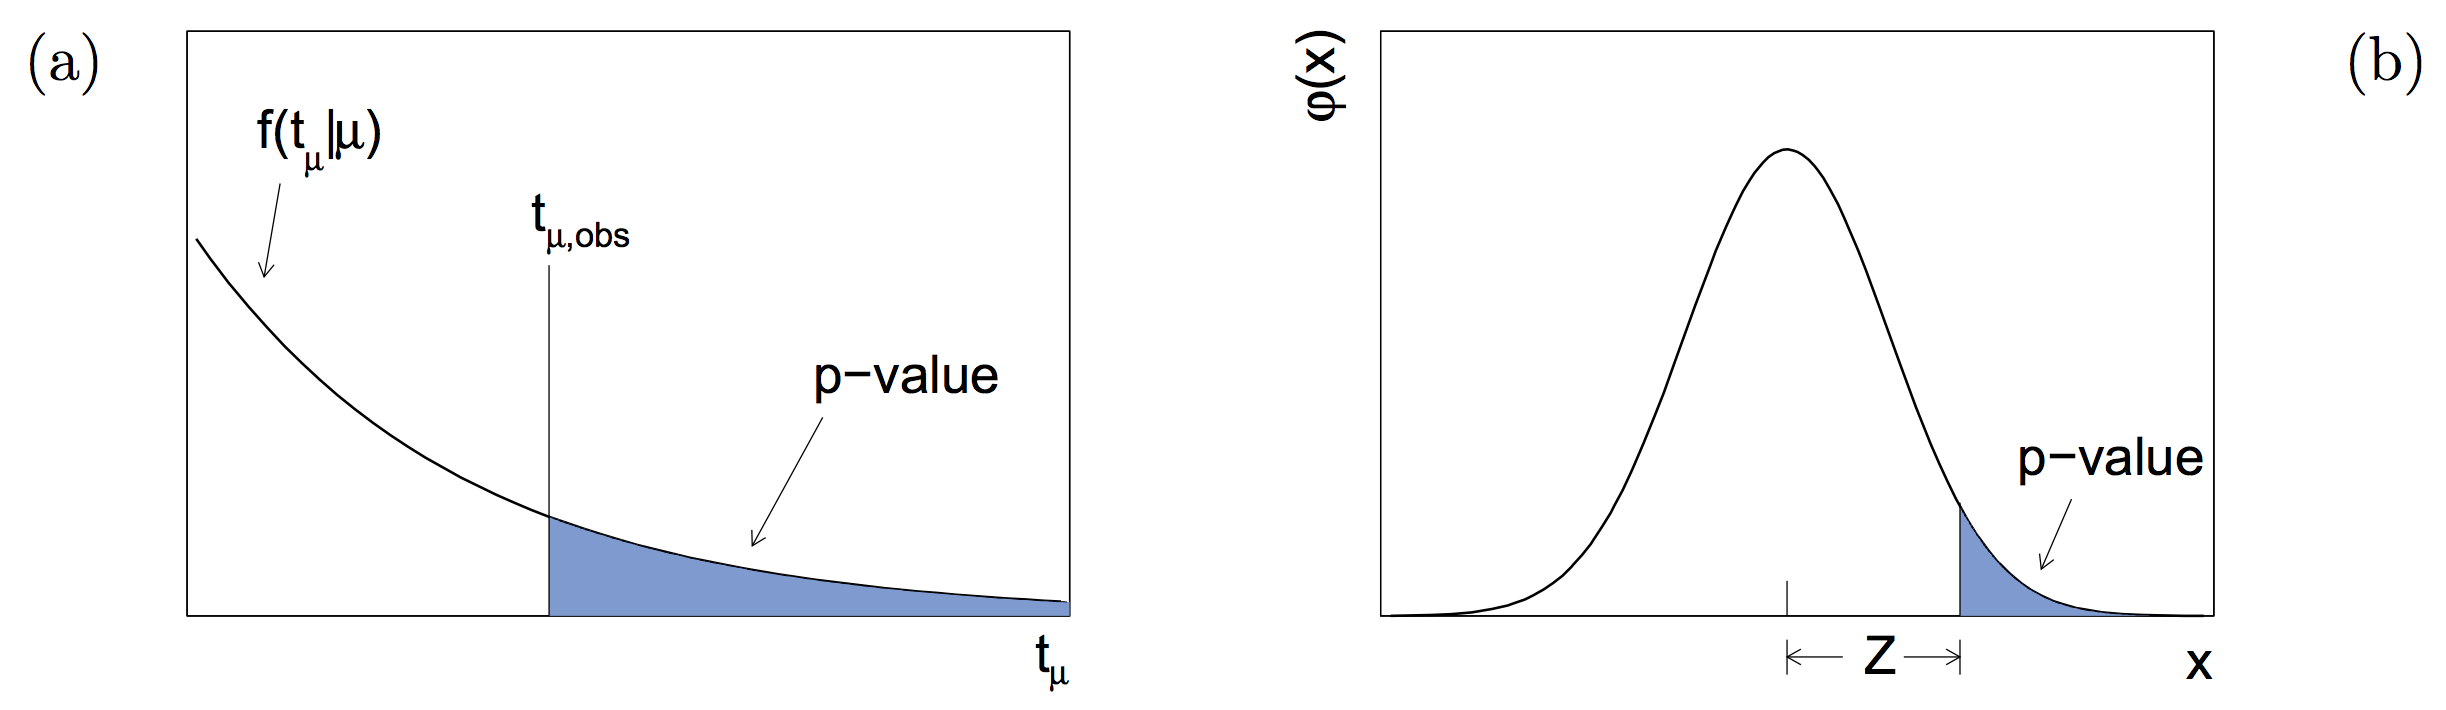
\includegraphics[width=1.0\textwidth]{figures/Statistic/test_statistic_pvalue_Z.png}
\end{center}
\caption{(a) Illustration of the relationship between the observed $t_{\mu}$ and its $p$-value. 
         (b) The relationship between $p$-value and the observed significance $Z$, where $\phi(x)$ is a standard normal distribution.
        }
\label{fig:pvalue_Z}
\end{figure}

In most cases, one assumes that the presence of a new signal can only increase the event rate comparing to the background only model,
then the signal strength $\mu \ge 0$.
And for the case of discovery, the hypothesis of a positive signal strength should be tested against to the background-only (null) hypothesis by using the test statistic called $p_0$:
\begin{equation}
    p_0 = 
    \begin{cases}
        -2 ln(\lambda(0)) &\hat{\mu} \ge 0 \\
        0                 &\hat{\mu} < 0
    \end{cases}
\end{equation}
which corresponds to the $p$-value called $p_0$:
\begin{equation}
    p_0 = \int_{q_{0, obs}}^{\infty} f(q_0|0) d q_0
\end{equation}
to quantify the level of disagreement between the data and the null hypothesis ($\mu = 0$).

\section{The CLs upper limit}

For a signal hypothesized value $\mu$, one can compute the probability that this hypothesis (called S+B hypothesis) gives a \textbf{greater} test statistic value than the observed one $q_{obs}$ as:
\begin{equation}
    p_{s+b} = \int_{q_{obs}}^{\infty} f(q_{\mu}|\mu) d q_{\mu}
\end{equation}
In the meantime, the probability that the background-only hypothesis gives a \textbf{smaller} test statistic than observed data can also be calculated as:
\begin{equation}
    1 - p_{b} = \int_{-\infty}^{q_{obs}} f(q_{\mu}|0) d q_{\mu}
\end{equation}
Then we define the CLs~\cite{Read_2002} of a hypothesized value $\mu$ as:
\begin{equation}
    CLs = \frac{p_{s+b}}{1-p_{b}}
\end{equation}
For purpose of excluding a signal hypothesis, a threshold CLs of 0.05 is often used.
For this reason, usually under the circumstance that no significant derivation between data and background-only hypothesis is found,
one would like to find the value of hypothesized signal strength $\mu$ by requiring its $CLs = 0.05$ (called 95\% CLs upper limit) for exclusion. 

The sensitivity of an experiment to exclude a new signal process is quantified by \textit{median upper limit},
which is obtained using ``Asimov dataset".
The Asimov dataset is defined such that when one uses it to evaluate the estimators for all parameters, one obtains the true parameter values.
Moreover, it is useful to use Asimov dataset to compute how much the sensitivity is expected to vary, given the expected fluctuations in the data.
The $\hat{\mu}$ is assumed to follow a Gaussian distribution with a mean value of $\mu '$ and the standard deviation of $\sigma$.
First of all, the test statistic from profile likelihood ratio can be approximated as~\cite{Cowan:2010js}:
\begin{equation}
	-2 ln \lambda(\mu) = \frac{(\mu - \hat{\mu})^2}{\sigma^2} + \mathcal{O}(1/\sqrt{N})
\end{equation}
Given that the Asimov dataset corresponding to a signal strength $\mu'$, one finds:
\begin{equation}
	-2 ln \lambda_{A}(\mu) \approx \frac{(\mu - \mu')^2}{\sigma^2} = q_{\mu,A}
\end{equation}
where $q_{\mu,A} = -2ln\lambda_{A}(\mu)$ is the observed test statistic of Asimov dataset.
Then the standard derivation can be computed as:
\begin{equation}
	\sigma_A^2 = \frac{(\mu - \hat{\mu})^2}{q_{\mu,A}}
\end{equation}
In a special situation where one wants to find the median exclusion significance for the hypothesis $\mu$ assuming that there is no signal ($\mu' = 0$),
one gets:
\begin{equation}
        \sigma_A^2 = \frac{\hat{\mu}^2}{q_{0,A}}
\end{equation}

\section{Nuisance parameters}
\label{sec:NPs}

The expected numbers and pdf shapes of signal and background events also depend on a series of systematic uncertainties, 
which are described as a set of nuisance parameters (NPs).
As showed in equation~\ref{eq:likelihoodf}, $\pmb{\theta}$ is a set of NPs that plays as an additional ``penalty" term to likelihood function, 
which will increase the negative log likelihood when any nuisance parameter is shifted from its nominal value.
Usually those NPs are constrained by using Gaussian function with their estimated uncertainties provided by the experiment condition.

